\section{Durchführung und Aufbau}
\label{sec:Durchführung}

\subsection{Aufbau}

Es wird der Aufbau in \autoref{fig:aufbau} verwendet.\\
Der Helium-Neon-Laser erzeugt einen Strahl linear polarisiertes, monochromatisches Licht.
Dieser durchläuft einen einstellbaren Polarisationsfilter, der das Licht wahlweise senkrecht oder parallel polarisiert. \\
Dann trifft er auf einen Spiegel mit Silizium-Oberfläche, welcher auf einen Drehteller montiert ist.
Der Drehteller kann um die vertikale Achse rotiert werden, um den Einfallswinkel des Lichtstrahls auf die Silizium-Oberfläche 
zu variieren. \\ 
Die Intensität des dort reflektierten Lichtstrahls, wird von einem Photoelement mit angeschlossenem Amperemeter gemessen.\\


\begin{figure}
    \centering
    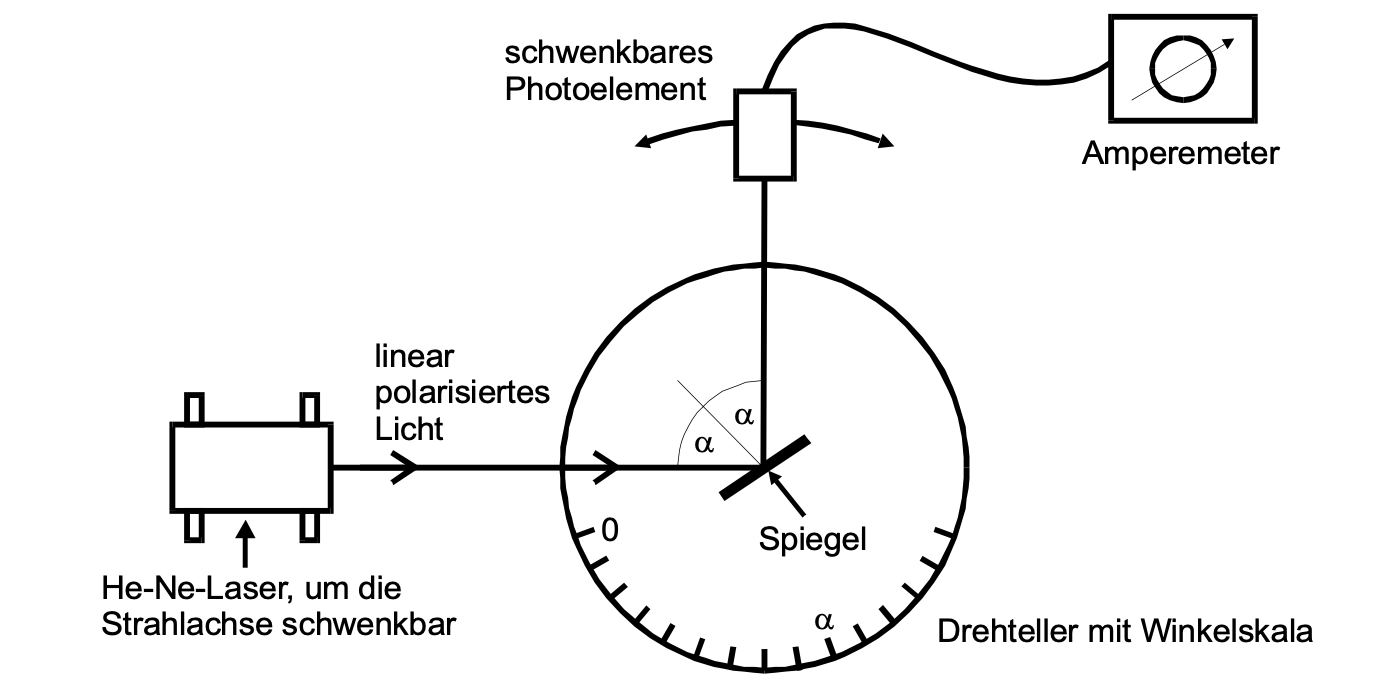
\includegraphics{content/aufbau}
    \caption{Die verwendete Messapparatur. \cite{sample}}
    \label{fig:aufbau}
  \end{figure}

  \subsection{Durchführung}
  Es wird jeweils für parallel und senkrecht polarisiertes Licht die Intensität gemessen, während der Einfallswinkel in 
  2° - Schritten von 2° bis 90° gesteigert wird. Zu diesem Zweck wird jeweils die auf dem Amperemeter angezeigte Stromstärke notiert.\\
  Anschließend werden noch der Dunkel- und Nullstrom gemessen. Beim Dunkelstrom ist der Laser ausgeschaltet, beim Nullstrom
  wird der Strahl nicht reflektiert.\\